\documentclass[parskip=half]{scrartcl}

\usepackage{xcolor}
\usepackage[hidelinks]{hyperref}
%\hypersetup{
%    colorlinks,
%    linkcolor={red!50!black},
%    citecolor={blue!50!black},
%    urlcolor={blue!80!black}
%}

\usepackage{graphicx}
\graphicspath{ {./images/} }

\usepackage{microtype}
\usepackage{fontspec}
\usepackage{unicode-math}

\usepackage[labelsep=period]{caption}
\newcommand\figref{Figure~\ref}

\let\oldFootnote\footnote
\newcommand\nextToken\relax

\renewcommand\footnote[1]{%
    \oldFootnote{#1}\futurelet\nextToken\isFootnote}

\newcommand\isFootnote{%
    \ifx\footnote\nextToken\textsuperscript{,}\fi}

\setmainfont{Georgia}
\setsansfont{Helvetica Neue}
\setmathfont{Stix Two Math}

\KOMAoptions{DIV=calc}

\begin{document}

\input{../author}

\begin{center}
    \Large
    \textsf{\textbf{Data Anonymisation}}
        
    \vspace{0.4cm}
    \large
    Homework 4: Privacy Preserving Technologies
        
    \vspace{0.4cm}
    \docauthor{}
       
    \vspace{0.9cm}
\end{center}

\tableofcontents

\section{Anonymisation Parameters}

In order to anonymise/pseudonymise the COVID-19 dataset provided to us, we need
to first define the rules according to which the ARX tool anonymises data. This
section describes the decisions in configuring these rules.

\subsection{Attribute Taxonomy}

Before starting the anonymisation procedure, we must determine the nature of
the different data attributes in the data set. Table~\ref{tab:attclass} shows
how we categorised each attribute.

\begin{table}
\begin{center}
    \begin{tabular}{ |l|l| } 
        \hline
        Attribute & Type\\
        \hline
        \hline
        id & Identifying\\
        \hline
        Age.at.diagnosis & Quasi-identifying\\
        \hline 
        Sex & Quasi-identifying\\
        \hline
        Native.country & Quasi-identifying\\
        \hline
        Month.first.diagnosis & Sensitive\\
        \hline
        Year.first.diagnosis & Sensitive\\
        \hline
        Vaccination & Quasi-identifying\\
        \hline
        Complicated.phase & Sensitive\\
        \hline
        Critical.phase & Sensitive\\
        \hline
        Last.known.patient.status & Quasi-identifying\\
        \hline
    \end{tabular}
    \caption{Attribute classification}
    \label{tab:attclass}
\end{center}
\end{table}

Naturally, an entry's identifier is identifying information, as it allows
directly identifying entries in the original dataset. We chose sex and native
country to be quasi-identifying, as these can be observed, found, or asked
about in everyday context. Information about the diagnosis, which we can
consider medical data, is typically sensitive and not public information about
an individual.

For two attributes the categorisation was less clear however. Namely, the age
at diagnosis could be considered medical data. Still, this age reveals the
minimum age of a person. Moreover, combined with the year/month of diagnosis,
an individual's birth-date could be narrowed down further. On their own, the
year and month of first diagnosis reveal little about a person. Hence, we argue
that age at diagnosis should be considered as a quasi-identifying attribute,
especially since age, or age-range, can be plausibly observed or determined.

The second unclear attribute is the last known patient status. While some
statuses such as ``recovered'' vs ``not recovered'' or the cause of death fall
under medical and therefore sensitive data, we argue that whether a person is
living or dead constitutes in quasi-identifying information, particularly since
in some countries or localities obituaries are common. Since there is
also statistical value in knowing whether a person died from COVID-19 or not,
we chose to consider last known patient status as quasi-identifying
information, to have greater control over the hierarchy levels.

We had an issue when considering last known patient data as a quasi-identifier
however. Namely, results were not satisfactory in that the generalisation
regarding age was too high. As such, to get better results, we changed
vaccination status to also be a quasi-identifier. This yielded far better
results, even if it may be more intuitive to consider vaccination information
as sensitive data. This concludes our attribute taxonomy.

\subsection{Privacy Models}

For quasi-identifying attributes, we chose the $10$-anonymity privacy model,
for which entries are only kept if there are at least $10$ entries with the
same quasi-identifying attributes. This provides some indistinguishability
guarantees for quasi-identifying attributes, as one would have at most a $1/10$
chance of correctly identifying an entry by guessing from the set.

For sensitive attributes, we used the distinct-$2$-diversity privacy model, as
an $l$-diversity model complements $k$-anonymity well. $2$-diversity means that
there are at least $2$ entries that are different combinations of equivalent
quasi-identifying attribute values for the given sensitive attribute. In other
words, for all records with the same quasi-identifying attribute values, there
must be at least $2$ entries with different values for the given sensitive
attribute. This is useful to prevent inferring sensitive information about a
person knowing only that they have belong to the set of people with equivalent
quasi-identifying attributes.

More generally, we used a suppression level of $100$\%, and set the population
region to be Europe, although we suspect the latter did little for the
anonymisation process.

\subsection{Hierarchy Rationale}

We note that when we describe the number of created levels, we describe the
number in addition to the ``level $0$'', where there is no grouping.

\subsubsection{Age at Diagnosis}

The age at diagnosis is numerical data, and is well suited for intervals. To
determine suitable intervals and clusters, we observed the distribution of
values. \figref{fig:age-distribution} displays the distribution of the age at
diagnosis, with values ranging from $1$--$94$.

\begin{figure}[ht]
    \begin{center}
        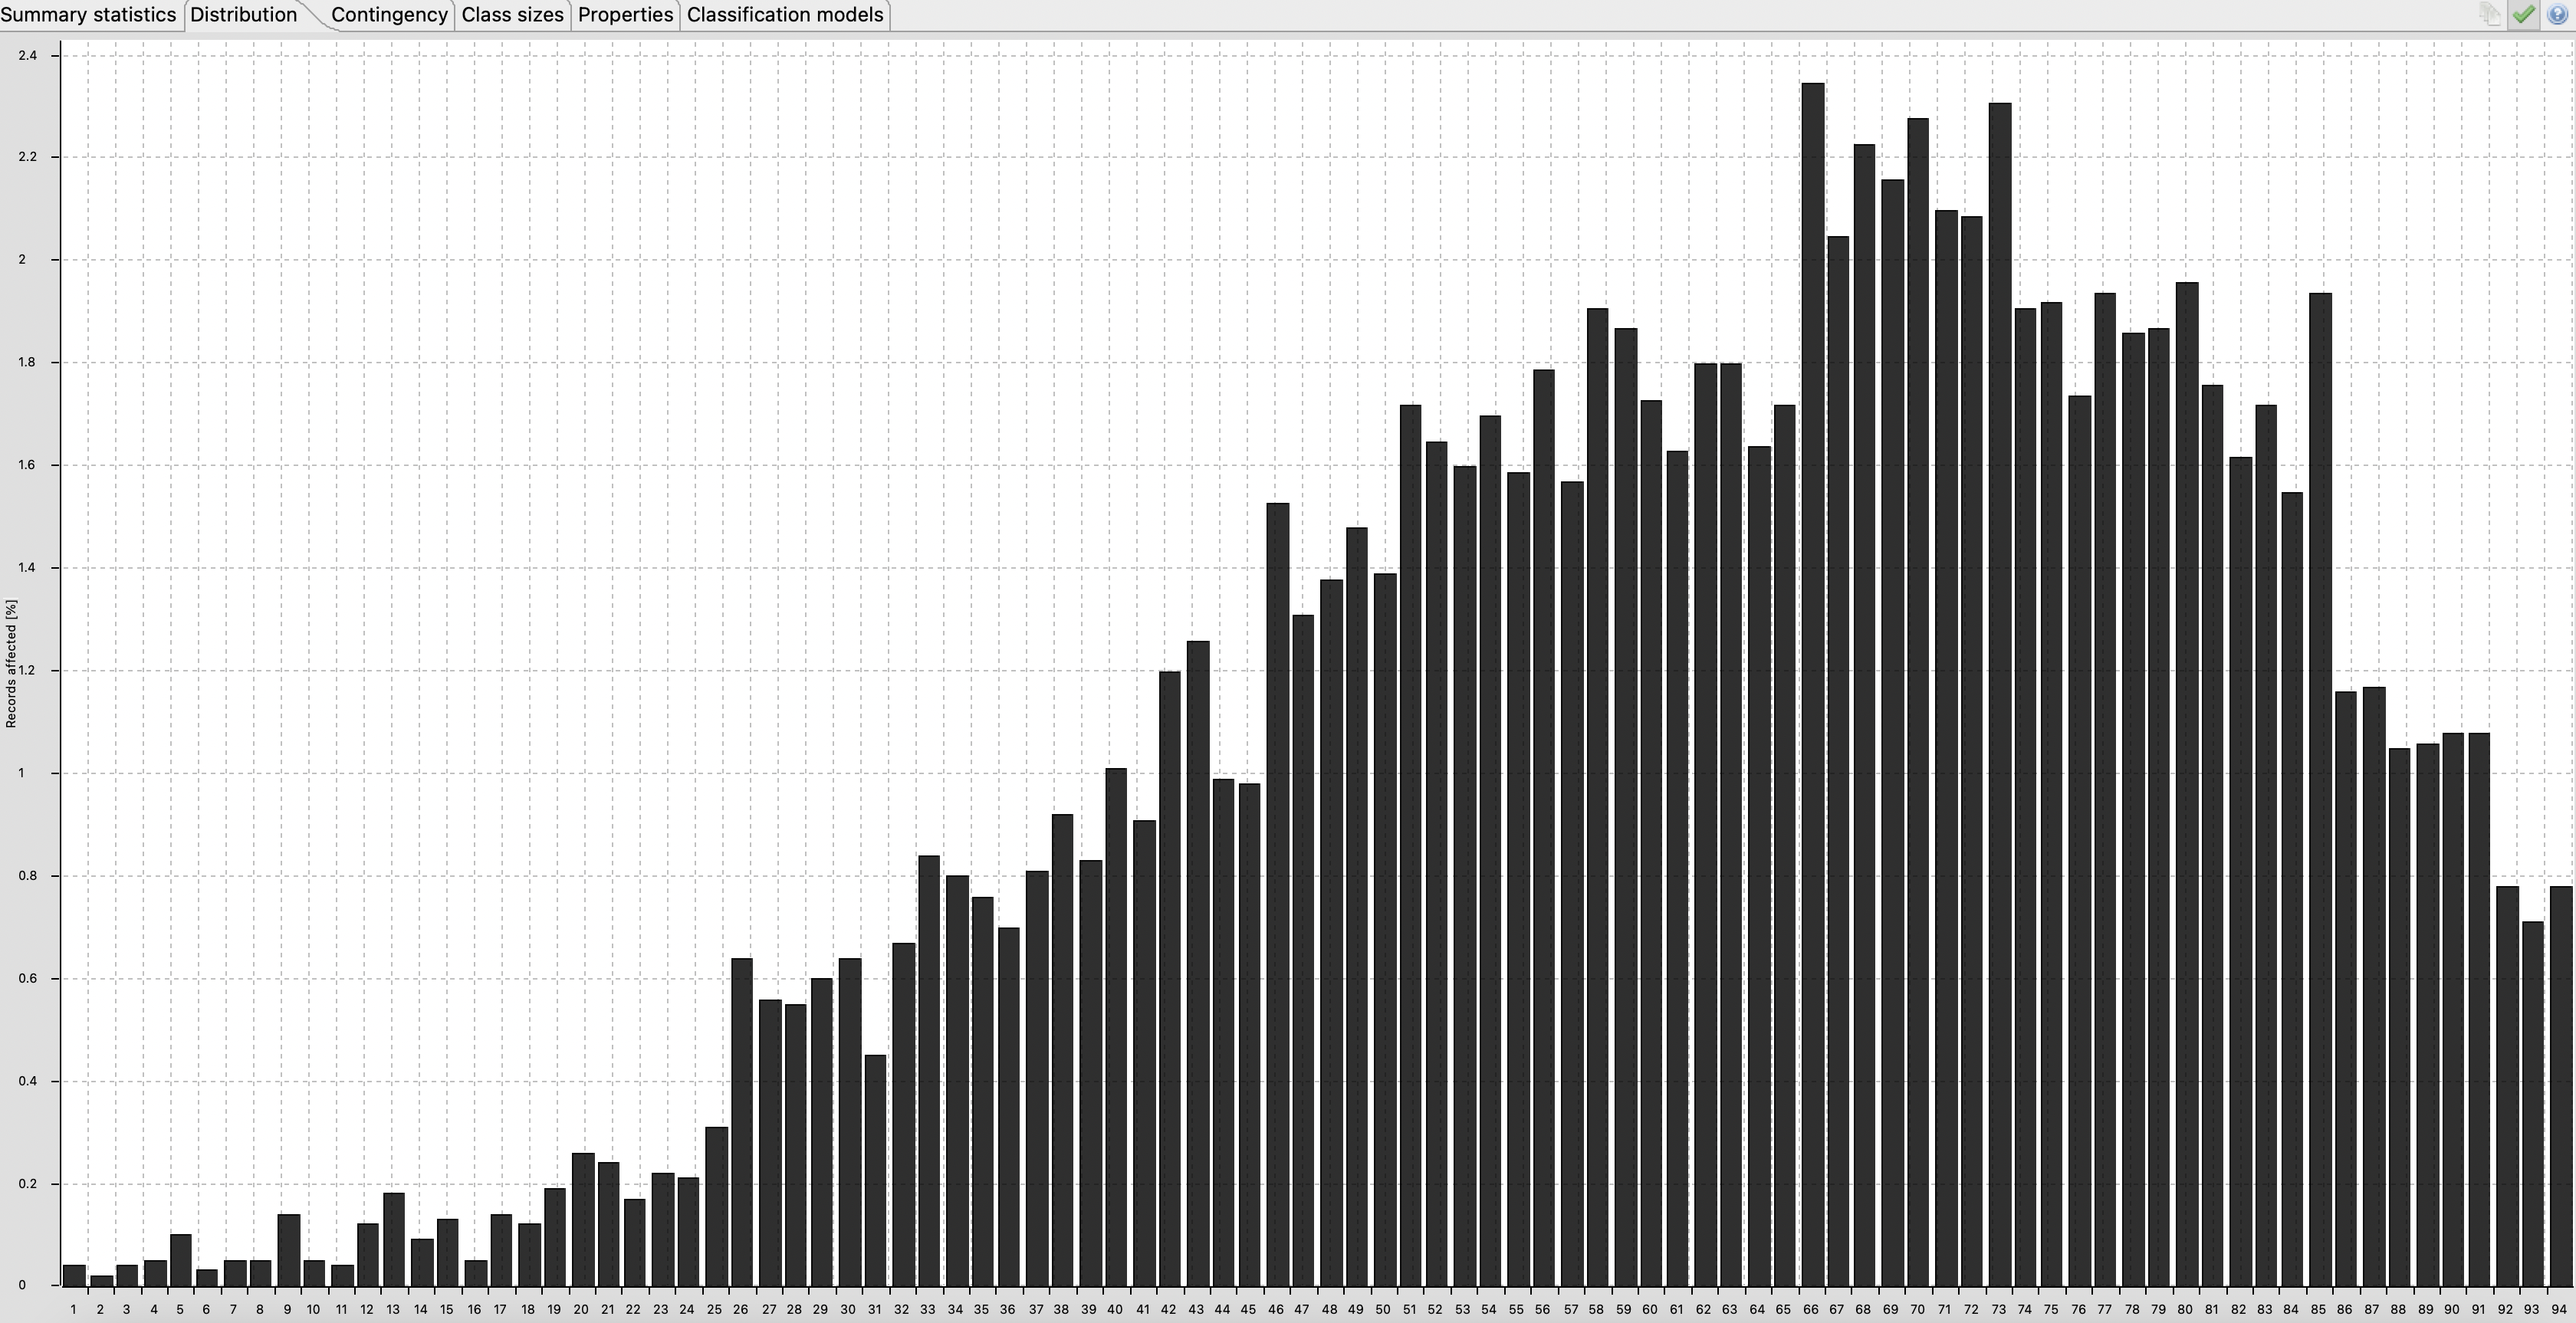
\includegraphics[width=\textwidth]{age_distribution}
        \caption{Distribution of age at diagnosis}
        \label{fig:age-distribution}
    \end{center}
\end{figure}

We observe that comparatively, there is only a small percentage of individuals
below the age of $26$ that were diagnosed. We hence decided to cluster together
ages $25$ and below, and to proceed in intervals of $5$ for the first level of
generalisation. Five levels of generalisation are hence created, with the
hierarchy shown in \figref{fig:age-intervals}.

\begin{figure}[ht]
    \begin{center}
        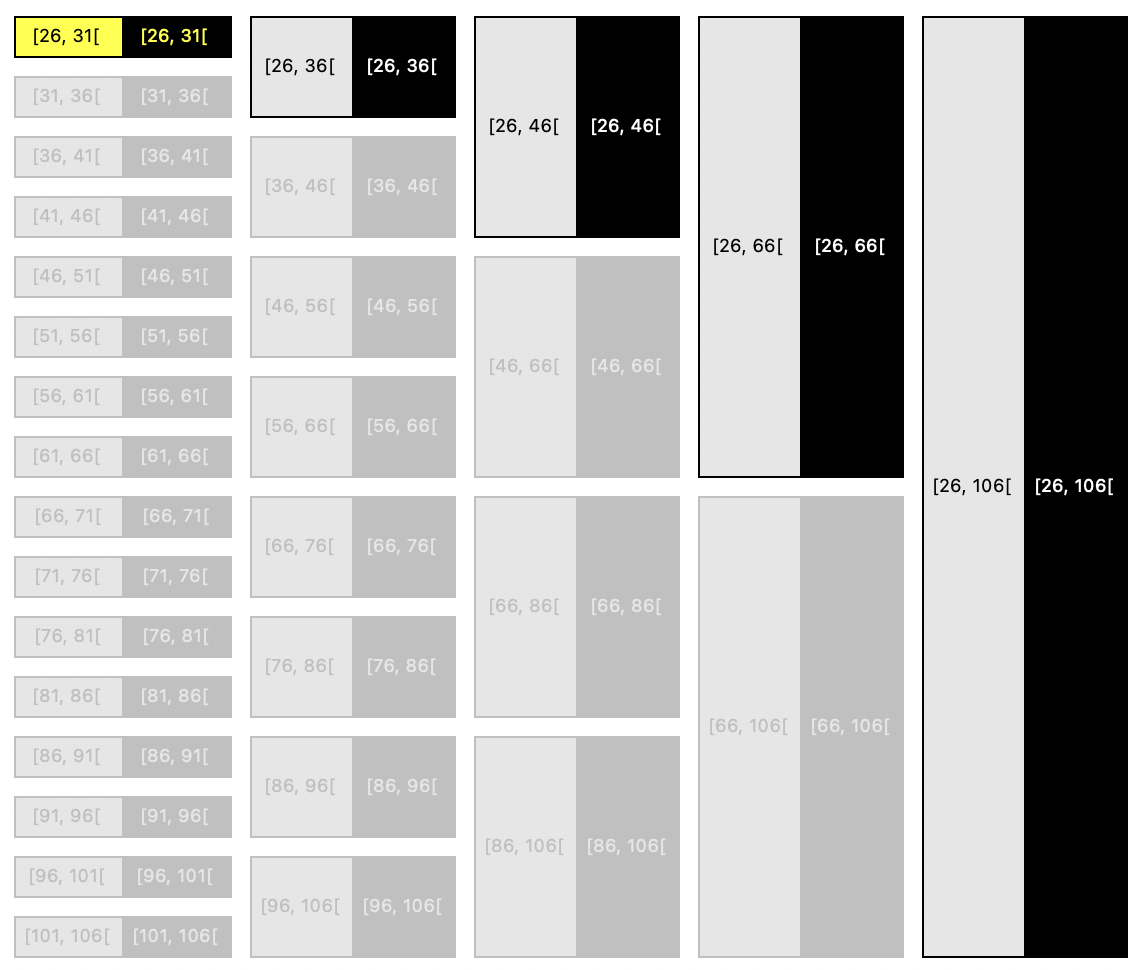
\includegraphics[width=200pt]{age_clusters}
        \caption{Hierarchy intervals for age at diagnosis}
        \label{fig:age-intervals}
    \end{center}
\end{figure}

We chose to keep the next-to-last level, i.e., $1$--$25$ and $26$--$94$, as
there may be some value in comparing the youth with adults, should it come to
that level of generalisation.

\subsubsection{Sex}

As there are only two available values for the sex, we chose a priority-based
hierarchy with only two levels: male and female, or none, i.e., both values are
removed.

\subsubsection{Native Country}

For the native country, the value distribution shown in
\figref{fig:country-distribution} shows that there is an overwhelming amount of
data for Germany, with Switzerland being the second country for nationals of
which most data is available in the provided dataset. Spain and Turkey follow
suit, with proportions big enough for us to consider them.

\begin{figure}[ht]
    \begin{center}
        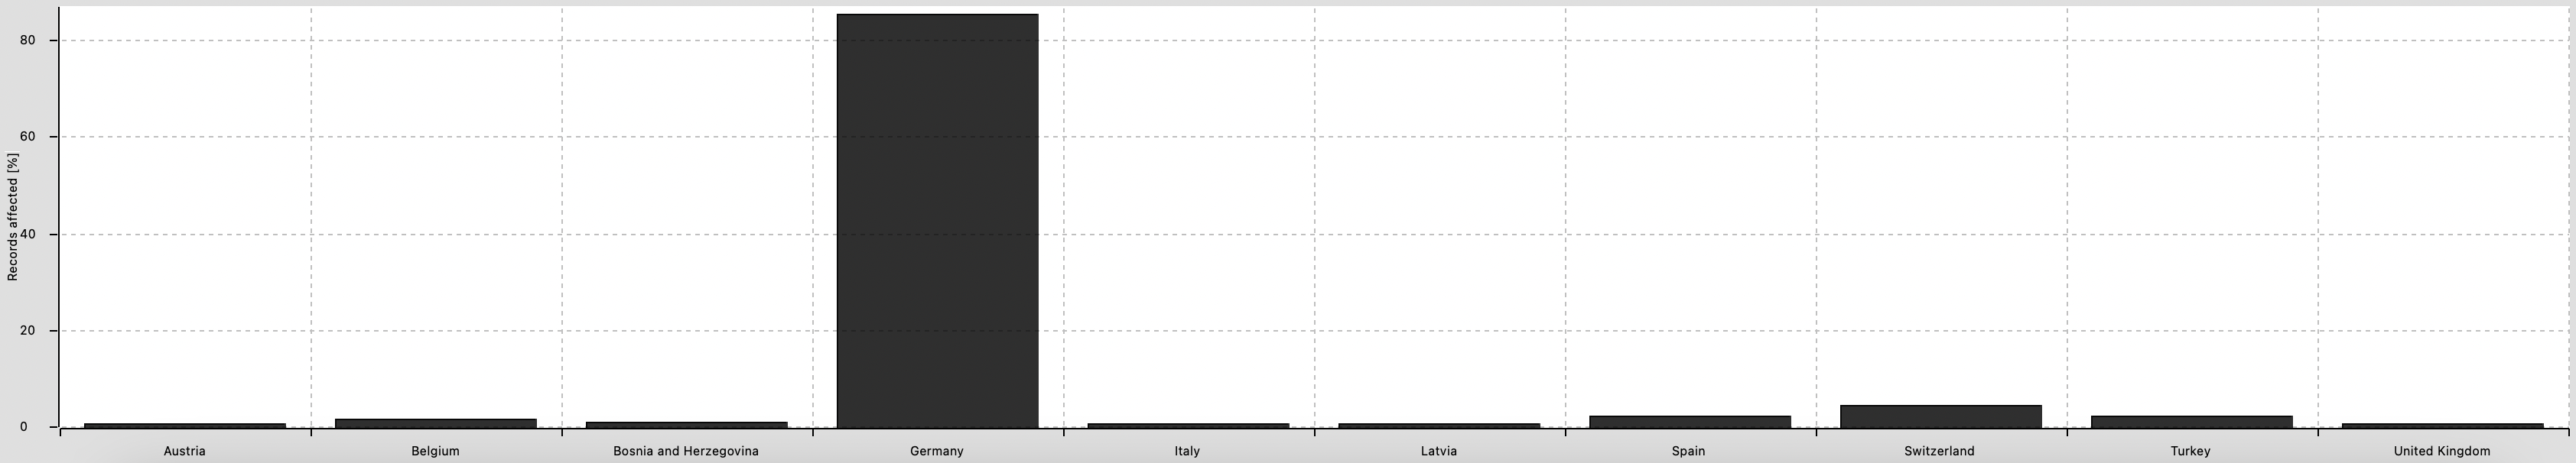
\includegraphics[width=\textwidth]{country_distribution}
        \caption{Distribution of native countries}
        \label{fig:country-distribution}
    \end{center}
\end{figure}

We hence decided on three levels of hierarchy: a first level for Germany,
Switzerland, Spain, Turkey, and others, a second level for Germany and others,
and a third level, where native countries are removed completely. We see no
value in pairing only Germany and Switzerland, and grouping the other countries
into one.

To achieve such a hierarchy, we used an ordering and grouping strategy, as
shown in \figref{fig:country-groups}, with the four most prominent native
countries ordered by number of records. The ordering of the remaining countries
does not matter, as we group them together in any case.

\begin{figure}[ht]
    \begin{center}
        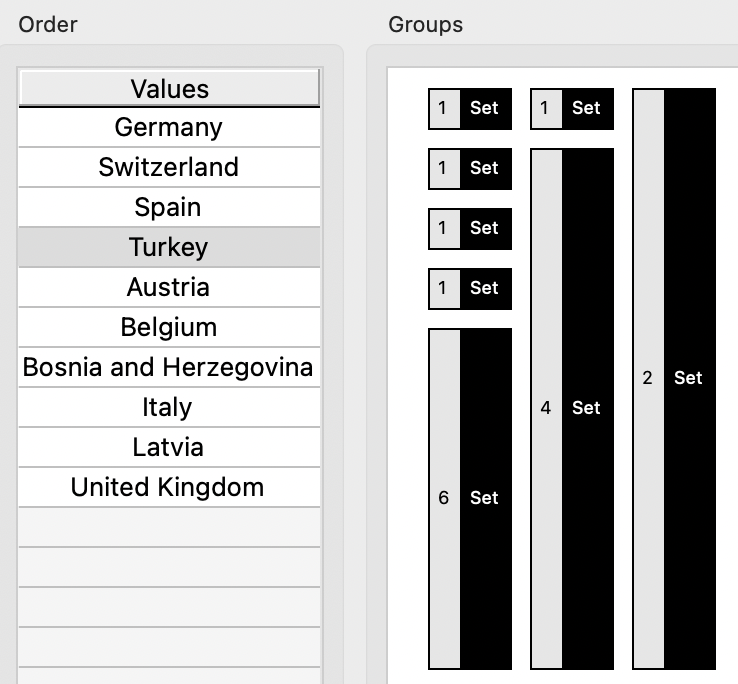
\includegraphics[width=200pt]{country_groups}
        \caption{Hierarchy groups of native countries}
        \label{fig:country-groups}
    \end{center}
\end{figure}

\subsubsection{Vaccination}

Regarding vaccination, it may be interesting to only mark whether a person
received any form of vaccination or not. Just in case, we consider also a
hierarchy group with vaccination information removed. We therefore created two
hierarchy levels using an ordering and grouping strategy, as shown in
\figref{fig:vaccination-groups}.

\begin{figure}[ht]
    \begin{center}
        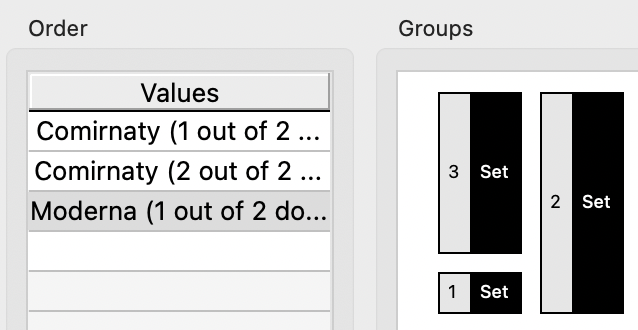
\includegraphics[width=250pt]{vaccination_groups}
        \caption{Hierarchy group for vaccination}
        \label{fig:vaccination-groups}
    \end{center}
\end{figure}

\subsubsection{Last Known Patient Status}

Regarding the last known status of patients, whether a person is dead or alive,
and whether the death was caused by COVID-19 or not would be interesting
information. Creating a hierarchy to match is slightly tricky, however, as
alive/dead and dead from COVID-19 provide different kinds of information. We do
not want to bundle deaths from other causes with unknown data, only to later
combine it with deaths, as this would lead to confusion.

Hence, we seek to create three levels of hierarchy: one where we pair together
alive individuals, a second where we distinguish only between alive, dead, and
unknown, and a third, where all values are removed. We used an ordering and
grouping strategy to achieve such a hierarchy, as shown in
\figref{fig:status-groups}.

\begin{figure}[ht]
    \begin{center}
        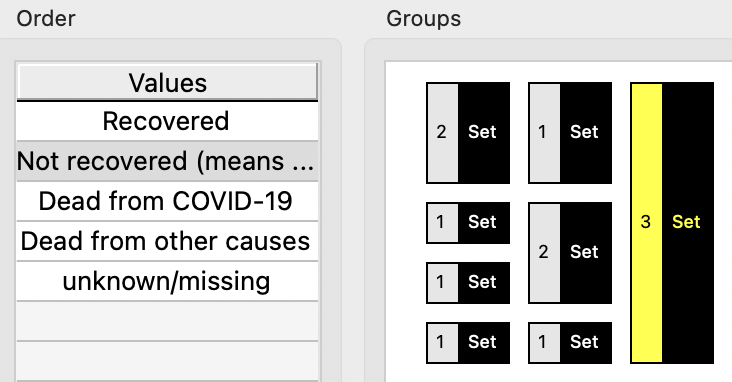
\includegraphics[width=250pt]{status_groups}
        \caption{Hierarchy groups for last known patient status}
        \label{fig:status-groups}
    \end{center}
\end{figure}

\section{Results}

In this section we describe the results of the anonymisation according to our
chosen parameters.

\subsection{Transformation Choice}

After applying the anonymisation criteria, the ARX tool provided us with a set
of potentially viable transformations shown in
\figref{fig:transformation-lattice}.

\begin{figure}[ht]
    \begin{center}
        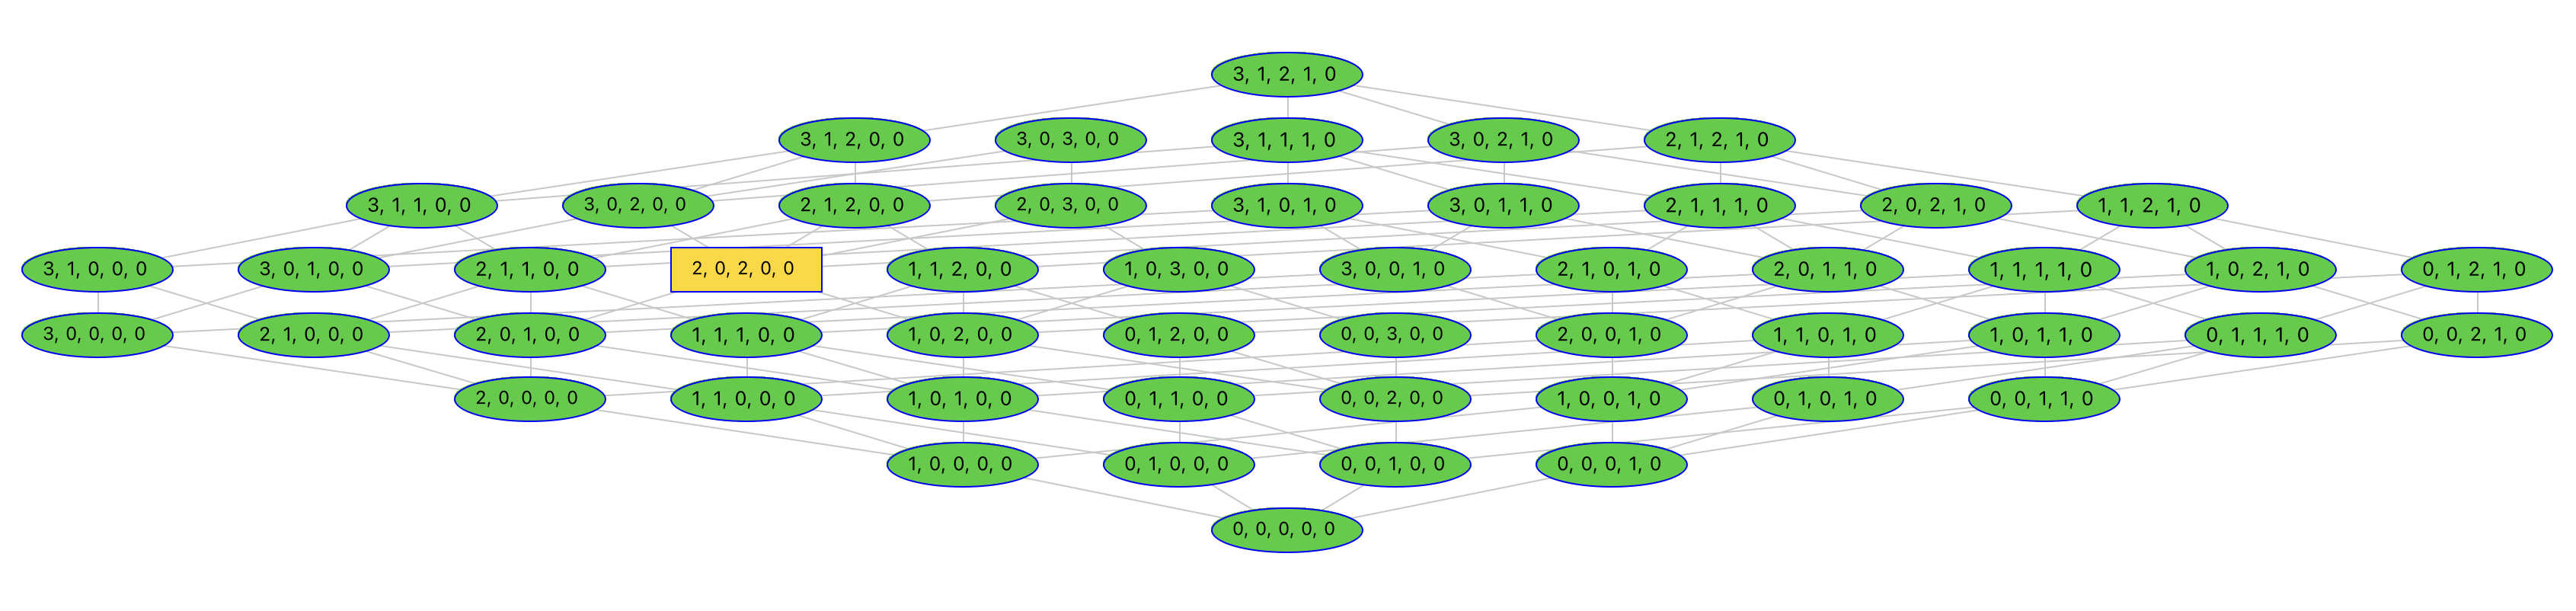
\includegraphics[width=\textwidth]{transformation_lattice}
        \caption{Lattice of proposed transformations}
        \label{fig:transformation-lattice}
    \end{center}
\end{figure}

We chose the transformation labelled as ``Optimum in category utility'' as it
showed the best results (according to scoring), as shown in
\figref{fig:transformation-scores}. Interestingly, it seems that a level 1
transformation regrading vaccination does not change the score, provided that
other levels are the same.

\begin{figure}[ht]
    \begin{center}
        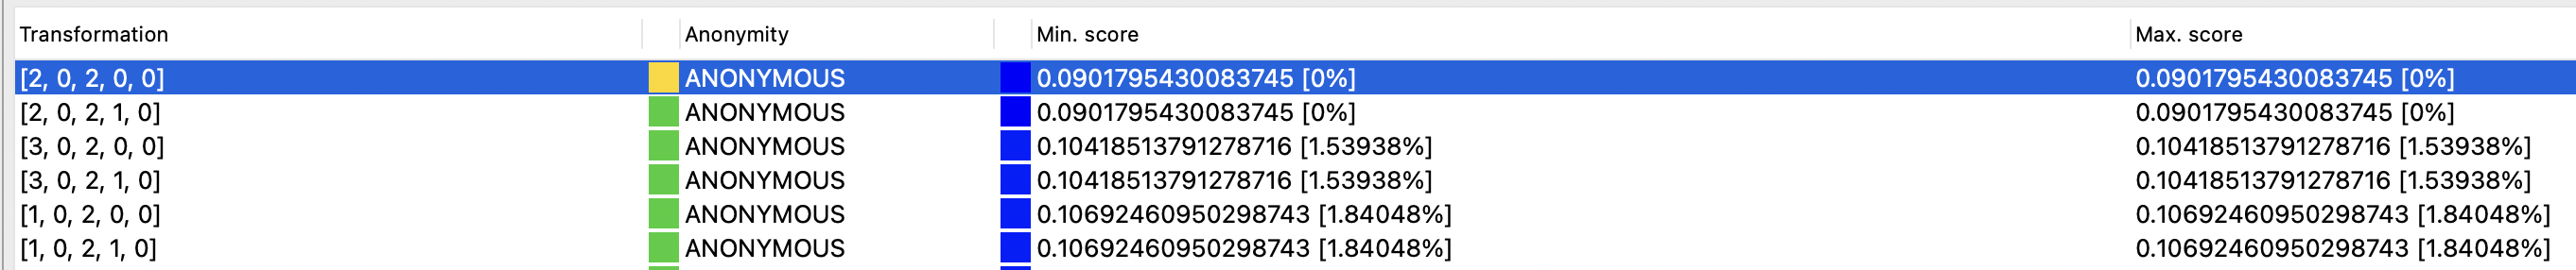
\includegraphics[width=\textwidth]{transformation_scores}
        \caption{Transformation scores}
        \label{fig:transformation-scores}
    \end{center}
\end{figure}

The chosen transformation applies a [2, 0, 2, 0, 0] transformation to the data,
which means that for the age at diagnosis, $10$-year intervals are chosen, and
regarding native countries, any country that is not Germany is bundled
together. For other quasi-identifiers, all values are kept.

More explicitly, the following transformation levels were applied:
\begin{itemize}
    \item age at diagnosis: level 2,
    \item sex: level 0,
    \item native country: level 2,
    \item vaccination: level 0,
    \item last known patient status: level 0.
\end{itemize}

\subsection{Analysis}

We describe the results of the applied transformations.

\subsubsection{Performance and Quality}

For the chosen levels, $672$ transformations were applied in total. The initial
minimal class size was $1$, and the minimal class size after transformations is
$10$.

In total, $493$ records, or $4.92$\% of all records, were suppressed. We
consider this an acceptable suppression ratio. The attribute with the most
missing values is the native country, with around $18$\% of missings. All
other quasi-identifying attributes share the same percentage of missing values,
which is around $5$\%. \figref{fig:quality} shows the ARX tool's quality
statistics.

\begin{figure}[ht]
    \begin{center}
        \includegraphics[width=\textwidth]{quality}
        \caption{Dataset quality scores}
        \label{fig:quality}
    \end{center}
\end{figure}

\subsubsection{Risks}

The risk of de-anonymisation with the input data is high. In fact, the models
project that some records could be de-anonymised with $100$\% probability.
More generally, about $8$\% of records have a risk of re-identification above
$50$\%, as read from the graph in \figref{fig:reid-risk-og}.

\begin{figure}[ht]
    \begin{center}
        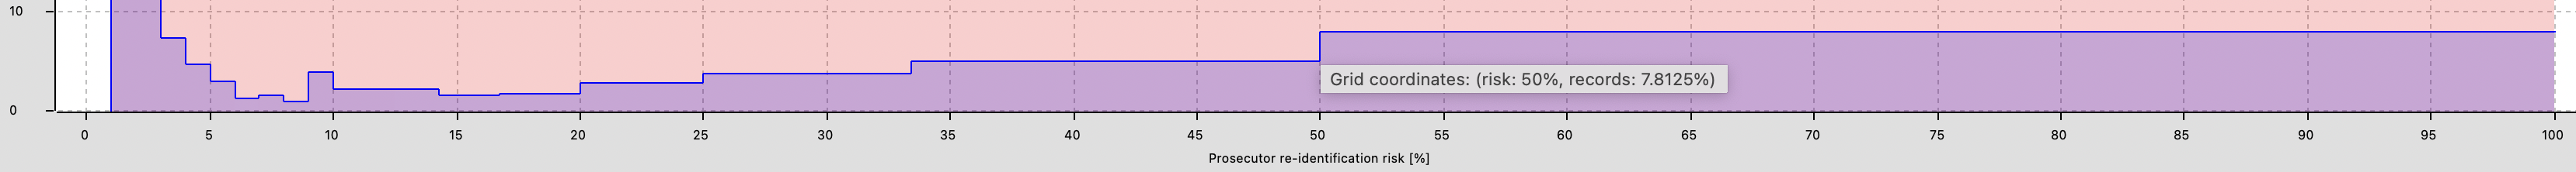
\includegraphics[width=\textwidth]{reid_risk_original}
        \caption{Risk of re-identification in original dataset}
        \label{fig:reid-risk-og}
    \end{center}
\end{figure}

From the risk graph for our anonymised, data, we read that around $98.6$\% of
records have a risk of re-identification below $5$\%, as shown in
\figref{fig:reid-risk-anon}.

\begin{figure}[ht]
    \begin{center}
        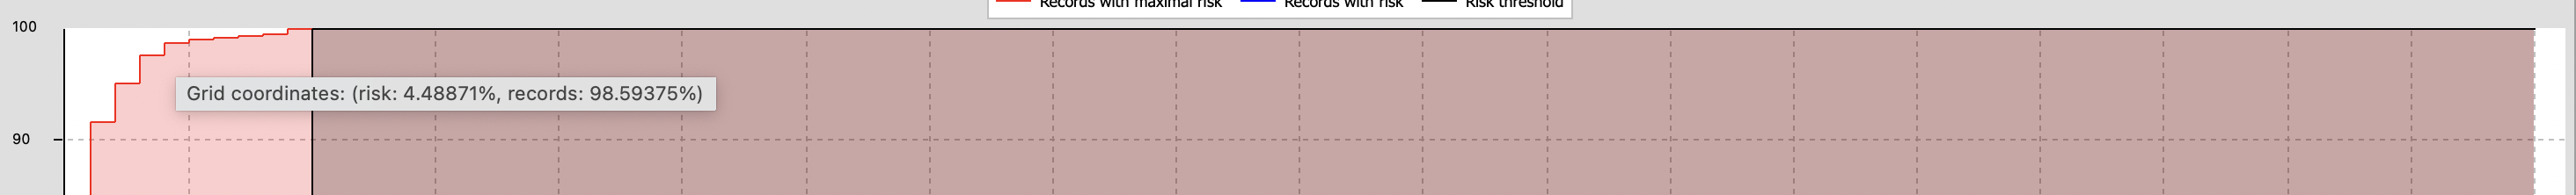
\includegraphics[width=\textwidth]{reid_risk_anon}
        \caption{Risk of re-identification in anonymised dataset}
        \label{fig:reid-risk-anon}
    \end{center}
\end{figure}

Combined with the data quality statistics, we conclude that our chosen model
provides good, though not perfect anonymity while retaining decent dataset
usability.

\textit{Previous attempt.} We note that had we considered vaccination and
last known patient status as sensitive attributes instead of quasi-identifying,
we would have reduced risks even further, however at the cost of a slightly
worse dataset quality.

\end{document}
